\section{Electric charge neutrality}
\label{section: charge neturality}


A pion condensate will have an electric charge.
In the grand canonical ensemble, the QCD Lagrangian will have the term  $\mu_Q \bar q \gamma^0 Q q$, where $\bar q \gamma^\mu Q q$ is the electric charge density, $Q$ the quark charge matrix \autoref{three-flavor charge matrix}, and $\mu_Q = \mu_I + 2 \mu_S$ is the electric charge chemical potential.
In the case of $\mu_S = 0$, the charge density is thus
%
\begin{equation}
    n_Q = - e \pdv{\Eff}{\mu_Q} = e n_I.
\end{equation}
%
A realistic astrophysical object will not have a macroscopic electric charge.
Therefore, we will model pion stars with the additional constraint of charge neutrality by including charged leptons in the form of muons or electrons.
These leptons are free fermions, with an electric charge of $- e$.
We may therefore use the results from \autoref{section: cold fermi star} and \autoref{section: fermions}.
The electric charge density of the leptons is given $- e n_\ell$, where $n_\ell$ is the particle number and, in this case, the lepton number.
In \autoref{Fermi gas particle density}, we found the expression
%
\begin{equation}
    \label{lepton density}
    n_{\ell} = \frac{8}{3} 
    \frac{u_{\ell, 0}}{m_\ell} x_f^3,
\end{equation}
%
where $x_f = \sqrt{ {\mu_\ell^2}/{m_\ell^2} - 1}$ is the dimensionless Fermi momentum, $m_\ell$ the lepton mass, and $\mu_\ell$ the lepton chemical potential.
This formula is valid for $\mu_\ell \geq m_\ell$.
We have introduced the characteristic energy density of leptons,
%
\begin{equation}
    u_{\ell, 0} = \frac{m^4_\ell}{3 \pi^2}.
\end{equation}
%
The criterion for charge neutrality is then
%
\begin{equation}
    \label{criterion charge neutrality}
    n_I = n_\ell.
\end{equation}
%
With this, we can determine the lepton chemical potential as a function of the isospoin chemical potential, $\mu_\ell = \mu_\ell(\mu_I)$.
The leading order result for the isospin density of the pion condensate is given in \autoref{isospin density}.
Inserting the expressions for these densities into \autoref{criterion charge neutrality}, we get
%
\begin{equation}
    \label{equation mu ell mu I}
    A \left(\frac{\mu_\ell^2 }{m_\ell^2} - 1 \right)^{3/2}
    = \frac{\mu_I}{m_\pi}\left( 1 - \frac{m_\pi^4}{\mu_I^4}  \right).
\end{equation}
%
Both densities vanish at the point $(\mu_I, \mu_\ell) = (m_\pi, m_\ell)$, which we have seen earlier is the point where the pressure and energy density of both the Fermi gas and the pion condensate vanish.
We have introduced the dimensionless constant
%
\begin{equation}
    A = \frac{3}{8} \frac{m_\pi} {m_\ell} \frac{u_{0, \ell}}{u_0}
    = \frac{1}{8 \pi^2} \frac{m_\ell^3}{m_\pi f_\pi^2}.
\end{equation}
%
Setting the lepton mass equal the electron mass or muon mass gives, respectively, $A = 1.360 \times10^{- 7}$ and $A = 5.709 \times 10^{3}$.
In this case, we can write the expression for $\mu_\ell(\mu_I)$ as an explicit function,
%
\begin{equation}
    \label{mu ell from mu I}
    \frac{\mu_\ell}{m_\ell}
    =
    \sqrt{
        1 + A^{-2/3}
        \left[
            \frac{\mu_I}{m_\pi}\left( 1 - \frac{m_\pi^4}{\mu_I^4}  \right)
        \right]^{2/3}
    }.
\end{equation}
%
These relationships are illustrated in \autoref{fig: chemical potentials}.
The plot on the left is the electron chemical potential as a function of isospin chemical potential, both normalized to the masses of their corresponding particles.
We see that the value of the electron chemical potential as a fraction of the particle mass is far greater than that of the pion condensate, as it is suppressed by the $A$ constant in \autoref{equation mu ell mu I}.
The muon chemical potential, shown on the right and normalized to the muon mass, is promoted by $A$ and thus much smaller than the isospin chemical potential.

\begin{figure}[!htb]
    \centering
    \begin{subfigure}{0.49 \textwidth}
        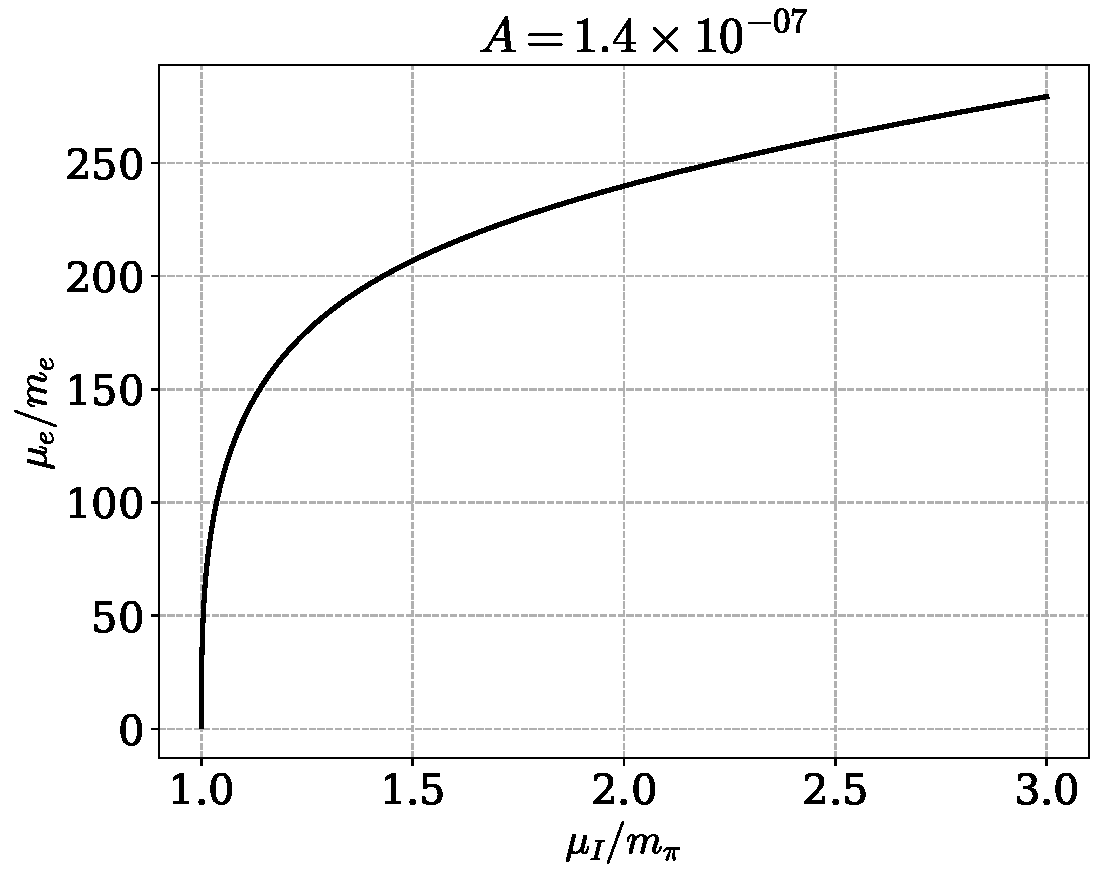
\includegraphics[width=\textwidth]{../scripts/figurer/charge_neutrality/chemical_potential_e.pdf}
    \end{subfigure}
    \begin{subfigure}{0.49\textwidth}
        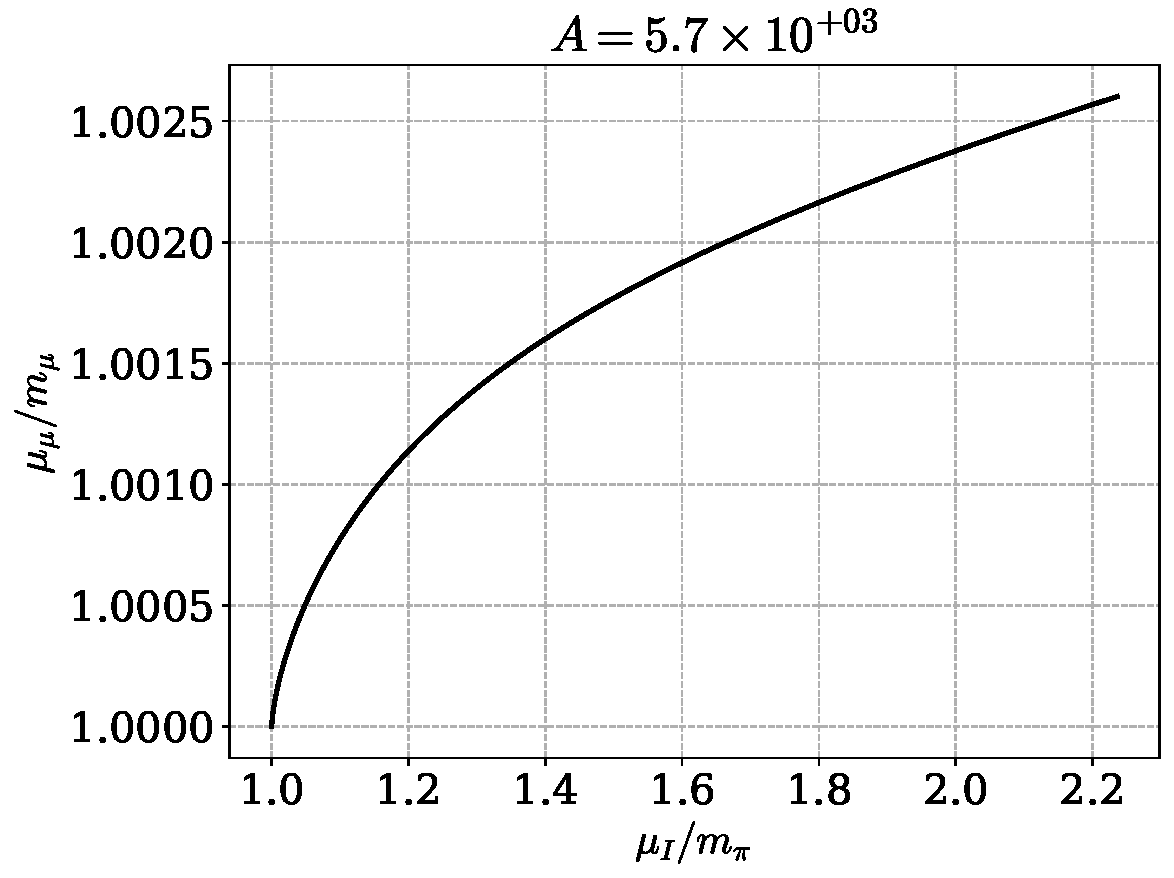
\includegraphics[width=\textwidth]{../scripts/figurer/charge_neutrality/chemical_potential_mu.pdf}
    \end{subfigure} 
    \caption{
        The lepton chemical potentials as functions of the isospin chemical potential, all normalized to their respective particles mass.
        The electron chemical potential is shown to the left, the muon to the right.
    } 
    \label{fig: chemical potentials}
\end{figure}


The total pressure and energy density will now be the sum of the contributions from the pion condensate and the leptons.
The lepton contribution to these, which we found in \autoref{Fermi gas energy density} and \autoref{Fermi gas pressure}, is
%
\begin{align}
    u_\ell 
    &= u_{\ell,0} 
    \left[(2x_f^3 + x_f) \sqrt{1 + x_f^2} - \arcsinh\left(x_f\right)\right], \\
    p_\ell
    &=\frac{1}{3} u_{\ell,0}
    \left[(2x_f^3 - 3x_f) \sqrt{1 + x_f^2} + 3\arcsinh\left(x_f\right)\right].
\end{align}
%
The contribution from the pion condensate is, as we found in \autoref{pressure leading order chpt} and \autoref{energy density leading order chpt},
%
\begin{align}
    u_\pi &= \frac{1}{2} u_0 \left( \frac{\mu_I}{m_\pi} - \frac{m_\pi}{\mu_I}\right)^2 \\
    p_\pi &= \frac{1}{2} u_0 \left( 2 + \frac{\mu_I^2}{m_\pi^2} - 3 \frac{m_\pi^2}{\mu_I^2}  \right)
\end{align}
%
This leads to a total pressure and energy
%
\begin{equation}
    p = p_\pi + p_\ell, \quad u = u_\pi + u_\ell.
\end{equation}
%
As \autoref{criterion charge neutrality} gives $\mu_\ell$ as a function of $\mu_I$, these are both parametrized by the isospin chemical potential, and we can extract the equation of state $u = u(p)$.
The full equation of state in two different regimes is show in \autoref{fig: eos with leptons}.
The plot on the left is the low-pressure regime.
As the light electron almost immediately enters the ultrarelativistic regime, defined by $\mu_e\gg m_e$, it will contribute mainly to the pressure.
On the other hand, the heavy muon is non-relativistic and thus contributes mainly to the energy density due to its rest mass.
On the right, we see that the ultrarelativistic limit is dominated by the pion contribution.

\begin{figure}
    \centering
    \begin{subfigure}{0.49\textwidth}
        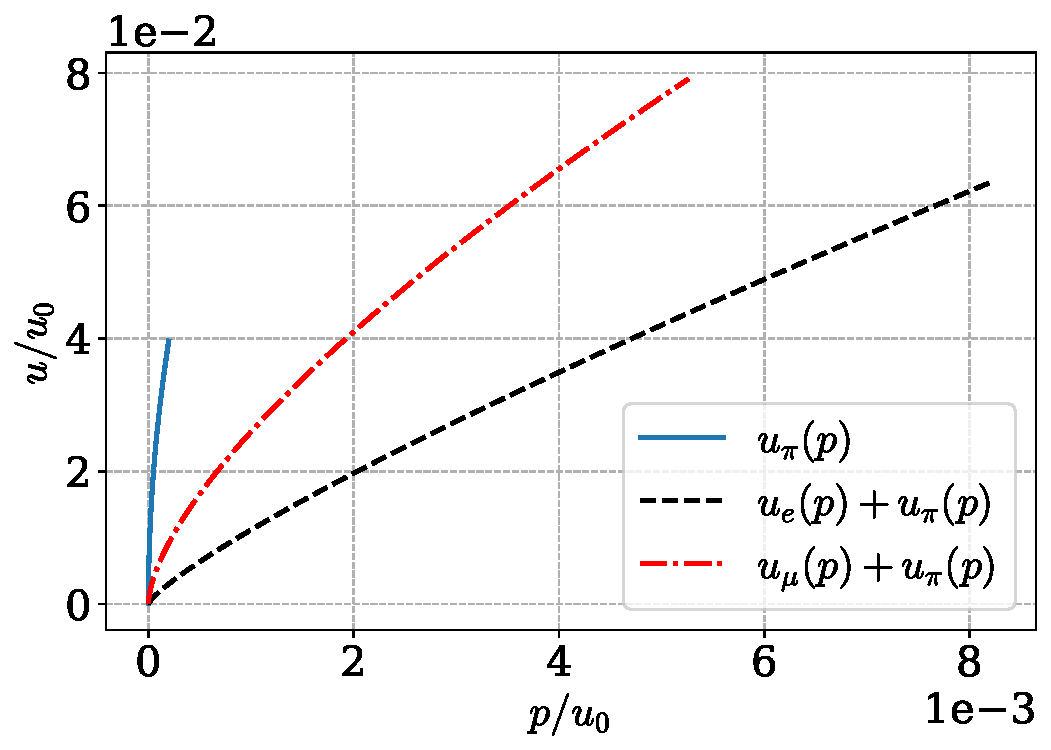
\includegraphics[width=\textwidth]{../scripts/figurer/charge_neutrality/eos_nr.pdf}
    \end{subfigure}
    \begin{subfigure}{0.49\textwidth}
        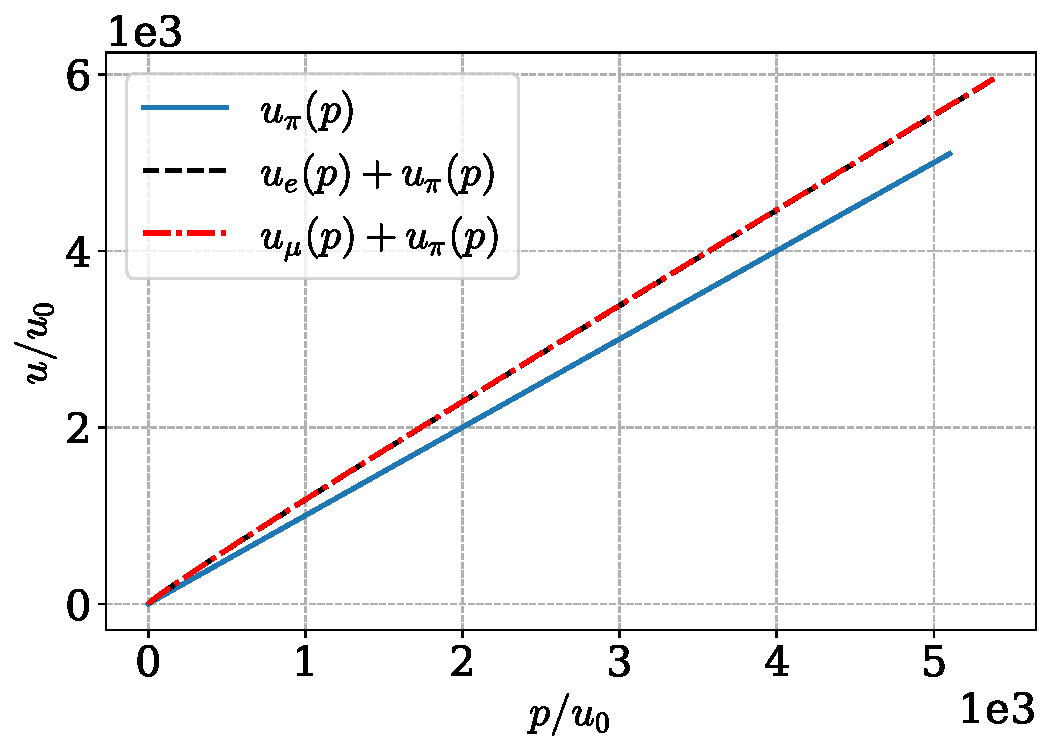
\includegraphics[width=\textwidth]{../scripts/figurer/charge_neutrality/eos_ur.pdf}
    \end{subfigure}
    \caption{
        The equation of state including a lepton is compared with the equation of state of only the pion condensate, in two different regimes.
        The pressure and energy density is normalized to $u_0 = f_\pi^2 m_\pi^2$.
    }
    \label{fig: eos with leptons}
\end{figure}


We can study the limit of the combined system, by again letting $\mu_I^2/m_\pi^2 = 1 + \epsilon$.
Inserting this into \autoref{mu ell from mu I} and expanding to first order in $\epsilon$, we get $\mu_\ell = 1 + (2 A^{-1} \epsilon)^{2/3} $.
This is equivalent to $x_f = (2 A^{-1} \epsilon)^{1/3} $.
In \autoref{section: cold fermi star}, we found the non-relativistic limit of the pressure and energy of the Fermi gas, i.e., the lowest order contribution in $x_f$, as $x_f \rightarrow 0$.
Inserting this new result into these limits, we get the leading low energy limits of the pressure and energy, 
%
\begin{equation}
    u_{\ell, \text{nr}} = \frac{8}{3} A^{-1} u_{\ell,0} \epsilon, \quad
    p_{\ell, \text{nr}} = \frac{8}{15} \left(\frac{2}{A} \right)^{5/3}  u_{\ell,0}  \epsilon^{5/3}.
\end{equation}
%
From \autoref{section: thermodynamics leading order}, we have the equivalent expressions for the pion condensate,
%
\begin{equation}
    u_{\pi, \text{nr}} = 2 u_0 \epsilon, \quad p_{\pi, \text{nr}} = \frac{1}{2} u_0 \epsilon^2.
\end{equation}
%
As we see, the energy density of the pion condensate and the leptons are of the same order, and will therefore both contribute to the leading order energy density.
However, the lepton pressure is of lower order, and \emph{only} this will contribute to the leading order pressure.
At low enough isospin chemical potential, then, the leading order behavior of the combined system is
%
\begin{equation}
    u_{\text{nr}} = 2 u_0 \left(1+ \frac{4}{3} \frac{u_{\ell,0}}{u_0} A^{-1} \right)\epsilon ,\quad
    p_{\text{nr}} = \frac{8}{15} u_{\ell,0} \left(\frac{2}{A} \right)^{5/3} \epsilon^{5/3}.
\end{equation}
%
The equation of state is now a polytrope with $\gamma = \frac{5}{3}$, different from the $\gamma = 2$ polytrope of only the pion condensate.
The equation of state of the lepton is compared with this limit in \autoref{fig: lepton eos}
This figure is not dependent on the mass of the lepton.

\begin{figure}
    \centering
    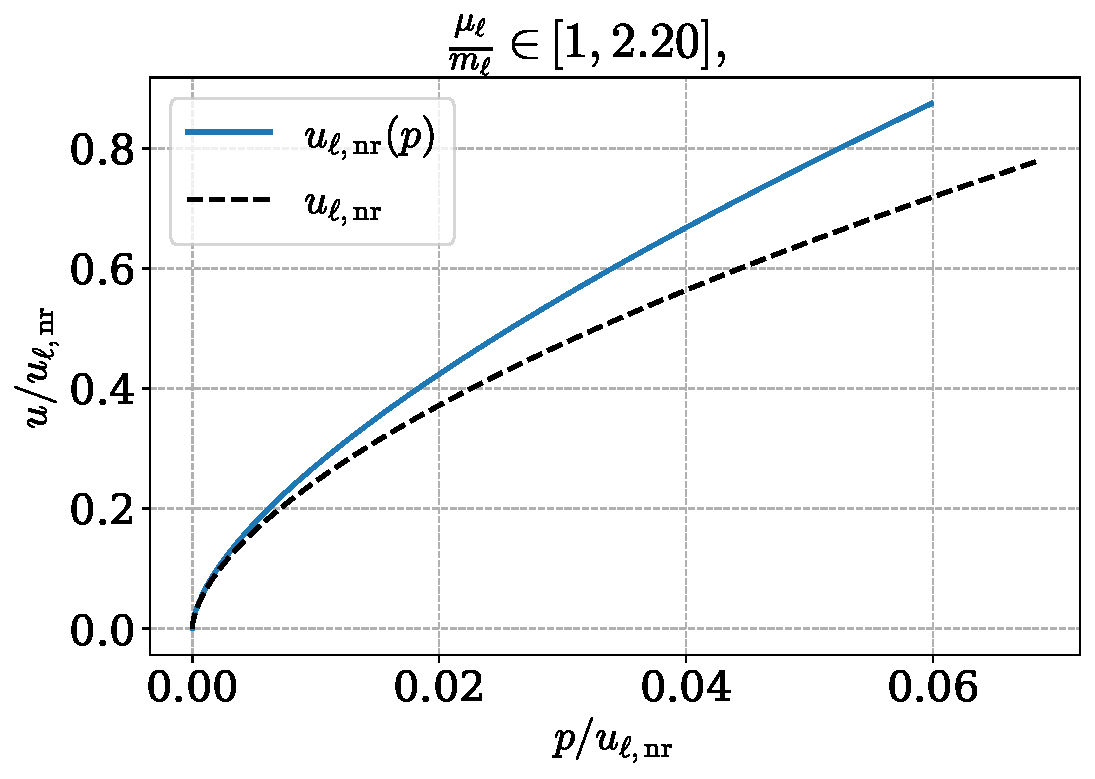
\includegraphics[width=0.6\textwidth]{../scripts/figurer/charge_neutrality/eos_lepton.pdf}
    \caption{The equation of state of the lepton, compared with the non-relativisitic limit.
    Both energy density and pressure are normalized to the characteristic lepton density.}
    \label{fig: lepton eos}
\end{figure}


In an intermediate range, however, the pressure of a heavy lepton will be suppressed by a factor $u_{\ell,0}/ u_0 A^{-5/3}\propto (m_\pi^{1/3} f_\pi^{{2}/{3}})^5 (m_\pi f_\pi)^{æ2} m_\ell^{-1}$, which for $m_\ell \gg m_\pi$ and $m_\ell \gg f_\pi$ is $\ll 1$, and the pion contribution might be dominant for a while.
In this regime, then, the equation of state is then still a polytrope with $\gamma = 2$, but the constant is changed due to the lepton contribution to the energy density.
The pressure in the intermediate range is
%
\begin{equation}
    p_i = \frac{1}{2} u_0 \epsilon^2,
\end{equation}
%
and the equation of state is thus
%
\begin{equation}
    p_i = K \left(\frac{u_\text{nr}}{u_0}\right)^2, \quad 
    K = \frac{1}{8} \left( 1 + \frac{4}{3} \frac{u_{\ell,0}}{u_0} A^{-1} \right)^{-2}.
\end{equation}

\begin{figure}[!htb]
    \centering
    \begin{subfigure}{0.49\textwidth}
        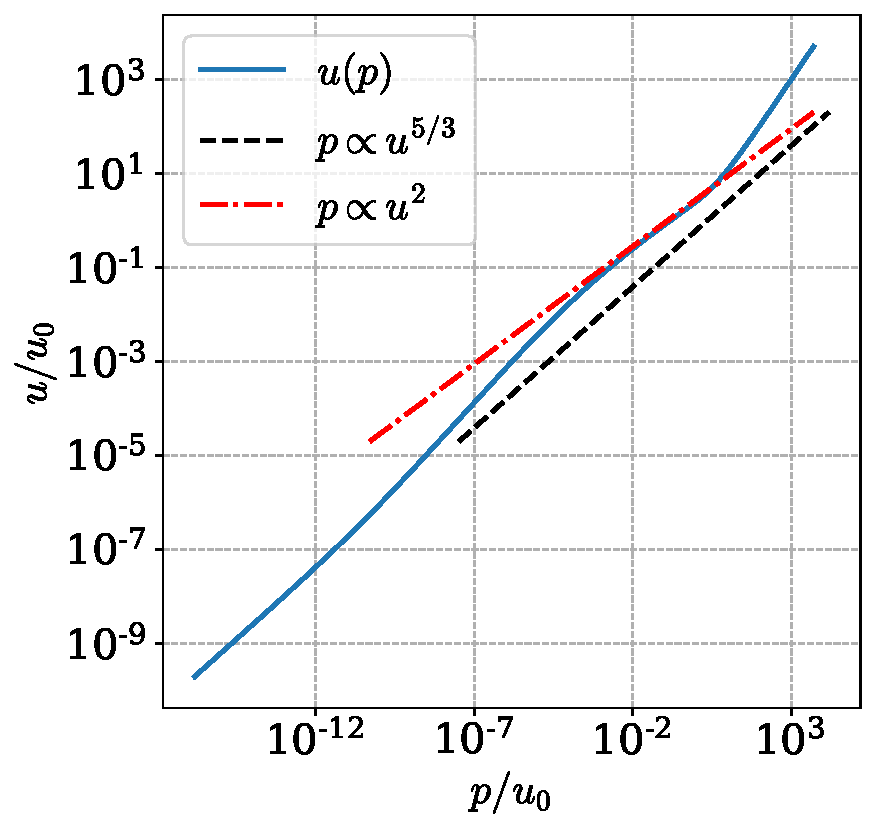
\includegraphics[width=\textwidth]{../scripts/figurer/charge_neutrality/eos_lepton_limitse.pdf}
    \end{subfigure}
    \begin{subfigure}{0.49\textwidth}
        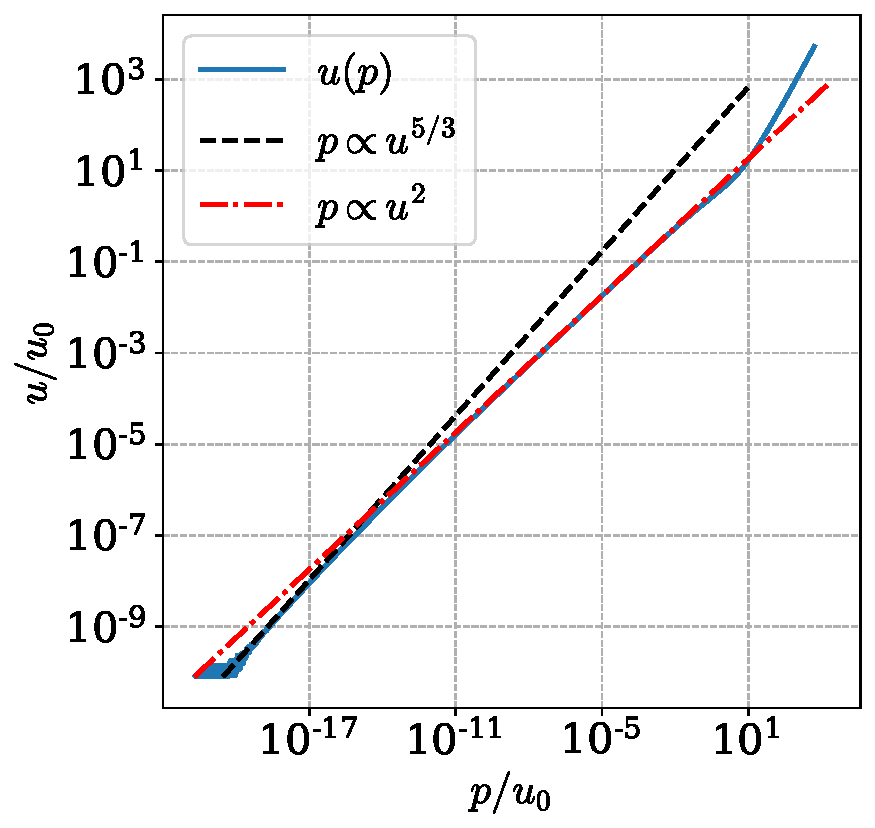
\includegraphics[width=\textwidth]{../scripts/figurer/charge_neutrality/eos_lepton_limitsmu.pdf}
    \end{subfigure}
    \caption{
        The full equation of state of the pion + lepton system, compared with intermediate and non-relativistic limit.
    On the right, the lepton is the electron, while on the left is the muon.
    The full equation of state is compared to two different limits.
    }
    \label{fig: intermediate regime}
\end{figure}

This is illustrated in \autoref{fig: intermediate regime}.
In this figure, both the intermediate limit and the non-relativistic limit is shown.
To the left is the system with electrons, and we see that even though $m_e < m_\pi$, there is still a regime of validity of around five orders of magnitude for the intermediate limit.
For $p/u_0 < 10^{-10}$, we see that the non-relativistic limit is very good.
On the right, we see that the intermediate limit has a very large range of applicability, of more than ten orders of magnitude.
The equation of state does finally approach the non-relativistic limit around $p/u_0 < 10^{-16}$, however it is necessary with higher-than-normal precision in the numerical calculations to see this.
 
We can find the ultrarelativistic regime by letting $\mu_I^2/m_\pi^2 = y$, $y \gg 1$.
From \autoref{mu ell from mu I}, we find that the lepton chemical potential to leading order in $y$ is $\mu_\ell^2 \propto y^{1/3}$.
I \autoref{section: cold fermi star}, we found that the ultrarelativistic limit of the Fermi both the pressure and energy is proportional to $x_f^4 \propto y^{2/3}$.
In the case of the pion, however, both are proportional to $\mu_I^2 \propto y$.
Therefore, the ultrarelativistic limit of the combined system is to leading order given by the ultrarelativistic limit of the pion condensate alone.

